\[\begin{tikzcd}[column sep=large]
	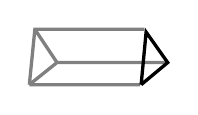
\begin{tikzpicture}[x=2em, y=2em]
    \draw[very thick, black!50]
        (0,0)--(2,0)
        (2.075,1)--(0.1,1)--(0,0)
        (0,0)--(0.5,0.4)--(0.1,1)
        (0.5,0.4)--(2.5,0.4);
	\draw[very thick] (2.02,0)--(2.5,0.4)--(2.11,0.95)--(2.02,0);
    \end{tikzpicture}
	 && A \\
	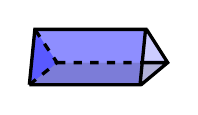
\begin{tikzpicture}[x=2em, y=2em,baseline=0.5em]
    \begin{scope}[very thick]
    \fill[fill=blue, opacity=0.3]
        (0,0)--(2,0)--(2.1,1)--(0.1,1)--(0,0);
    \fill[fill=blue!50!black, opacity=0.3]
        (0,0)--(0.5,0.4)--(2.5,0.4)--(2,0)--(0,0);
    \fill[fill=blue, opacity=0.2]
        (0.1,1)--(0.5,0.4)--(2.5,0.4)--(2.1,1)--(0.1,1);
    \fill[fill=blue, opacity=0.5]
        (0.1,1)--(0.5,0.4)--(0,0)--(0.1,1);
    \draw
        (0,0)--(2,0)--(2.1,1)--(0.1,1)--(0,0)
        (2.02,0)--(2.5,0.4)--(2.117,1.001)
        (2.05,0.4)--(2.5,0.4);
    \draw[dashed]
        (0,0)--(0.5,0.4)--(0.1,1)
        (0.5,0.4)--(2.05,0.4);
    \end{scope}
    \end{tikzpicture}
    && X \\
	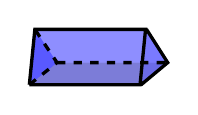
\begin{tikzpicture}[x=2em, y=2em,baseline=0.5em]
    \begin{scope}[very thick]
    \fill[fill=blue, opacity=0.3]
        (0,0)--(2,0)--(2.1,1)--(0.1,1)--(0,0);
    \fill[fill=blue!50!black, opacity=0.3]
        (0,0)--(0.5,0.4)--(2.5,0.4)--(2,0)--(0,0);
    \fill[fill=blue, opacity=0.2]
        (0.1,1)--(0.5,0.4)--(2.5,0.4)--(2.1,1)--(0.1,1);
    \fill[fill=blue, opacity=0.5]
        (0.1,1)--(0.5,0.4)--(0,0)--(0.1,1);
    \fill[fill=blue, opacity=0.4]
        (2,0)--(2.5,0.4)--(2.1,1);
    \draw
        (0,0)--(2,0)--(2.1,1)--(0.1,1)--(0,0)
        (2.02,0)--(2.5,0.4)--(2.117,1.001);
    \draw[dashed]
        (0,0)--(0.5,0.4)--(0.1,1)
        (0.5,0.4)--(2.5,0.4);
    \end{scope}
    \end{tikzpicture}
	\arrow["\bigcup\psi_{d_i^*(f)}{(-,e_1)}", from=1-1, to=1-3]
	\arrow[from=1-1, to=2-1]
	\arrow[from=2-1, to=3-1]
	\arrow["{\psi_f}"', from=3-1, to=2-3]
	\arrow["\lambda"', dashed, from=2-1, to=1-3]
\end{tikzcd}\]